%-------------------------------------------------------------------------
\documentclass[11pt,a4paper,colorlinks,breaklinks]{article}
%-------------------------------------------------------------------------

%-------------------------------------------------------------------------
\usepackage{calc}
\usepackage[text={16cm,23cm},centering=true,showframe=false]{geometry}
\usepackage{fancybox,fancyvrb,fancyhdr,lastpage,lineno,import}
\usepackage{longtable,multirow}
\usepackage{xcolor,graphics,xmpmulti,pgf,pgfpages,tikz,wrapfig}
\usepackage{colortbl,color}
\usepackage{amsmath,amssymb,amsfonts}
\usepackage{hyperref,multimedia,rotating,framed,pstricks}
\usepackage{listings,index}
%
%---- pdflatex
%\usepackage[T1]{fontenc}
%\usepackage[utf8]{inputenc}
%---- xelatex
\usepackage{fontspec}
%
\usepackage[french]{minitoc}
\usepackage[french]{babel}
\usepackage[french]{nomencl}
\usepackage[framed,hyperref,standard]{ntheorem}
\usepackage{eurosym,pifont}
%-------------------------------------------------------------------------

%-------------------------------------------------------------------------
\lstset
{
language=Python,
basicstyle=\ttfamily,
identifierstyle=\ttfamily,
keywordstyle=\color{blue}\ttfamily,
commentstyle=\color{gray}\ttfamily,
stringstyle=\color{green}\ttfamily,
showstringspaces=false,
extendedchars=true,
numbers=left, 
numberstyle=\color{blue}\tiny,
frame=lines,
linewidth=0.95\textwidth,
xleftmargin=5mm
} 
%-------------------------------------------------------------------------

%-------------------------------------------------------------------------
\pgfdeclareimage[width=3cm,interpolate=true]{logo-enib}{logo-enib}
%-------------------------------------------------------------------------

%-------------------------------------------------------------------------
\pagestyle{fancy}
\fancyhead{}
\fancyhead[L]{\hspace*{-3em}\begin{minipage}{3cm}\pgfuseimage{logo-enib}\end{minipage}}
\fancyhead[C]{Informatique S1 -- 2013-2014}
\fancyhead[R]{\thepage/\pageref{LastPage}}
\fancyfoot{}
\fancyfoot[L]{}
\fancyfoot[C]{}
\fancyfoot[R]{}
\setlength{\headheight}{40pt}
\setlength{\footskip}{38pt}
\renewcommand{\headrulewidth}{0pt}
\renewcommand{\footrulewidth}{0pt}
%-------------------------------------------------------------------------

%-------------------------------------------------------------------------
\input{sigle}
%-------------------------------------------------------------------------

\graphicspath{{../fig/}}

%-------------------------------------------------------------------------
\begin{document}
%-------------------------------------------------------------------------
\begin{center}
{\huge\bf Initiation à l'algorithmique}\\[3mm]
{\Large --- Organisation du cours ---}
\end{center}

Ce document présente les principales caractéristiques organisationnelles
du cours d'informatique de l'\enib{} au semestre S1.

%-------------------------------------------------------------------------
\section{Equipe pédagogique}
%-------------------------------------------------------------------------

\begin{tabular}{lllll}
Parenthoën & Marc       & \mc   & \href{mailto:parenthoen@enib.fr}{\texttt{parenthoen@enib.fr}} & (responsable)\\
\hline
Ben Ismail	& Sahbi		& \ater & \href{mailto:benismail@enib.fr}{\texttt{benismail@enib.fr}} \\
Jost		& Céline	& \ater	& \href{mailto:jost@enib.fr}{\texttt{jost@enib.fr}} \\
Kubicki		& Sébastien & \mc	& \href{mailto:kubicki@enib.fr}{\texttt{kubicki@enib.fr}} \\
Nédélec    & Alexis     & \mc   & \href{mailto:nedelec@enib.fr}{\texttt{nedelec@enib.fr}} \\
Tisseau    & Jacques    & \pr   & \href{mailto:tisseau@enib.fr}{\texttt{tisseau@enib.fr}}
\end{tabular}

%-------------------------------------------------------------------------
\section{Objectifs du cours}
%-------------------------------------------------------------------------


%-------------------------------------------------------------------------
\subsection{Objectifs thématiques}
%-------------------------------------------------------------------------
L'objectif principal des enseignements d'informatique S1 de l'\enib{}
est l'acquisition des \textbf{notions fondamentales de l'algorithmique}.
Plus précisément, nous étudierons successivement :
\begin{enumerate}
\item les instructions de base permettant de décrire les algorithmes : affectation, tests, boucles;
\item les procédures et les fonctions qui permettent de structurer et de réutiliser les algorithmes;
	on parlera alors d'encapsulation, de préconditions, de portée des variables, de passage de paramètres,
	d'appels de fonctions, de récursivité et de jeux de tests;
\item les structures de données linéaires : tableaux, listes, piles, files, qui améliorent la
	structuration des données manipulées par les algorithmes. A cette occasion, on évaluera
	la complexité et l'efficacité de certains algorithmes utilisant ces structures linéaires.
\end{enumerate}
Ces différentes notions seront \textbf{mises en \oe uvre à travers l'utilisation du 
langage \href{http://www.python.org/}{\python}}.



%-------------------------------------------------------------------------
\subsection{Objectifs pédagogiques}
%-------------------------------------------------------------------------
Au cours du semestre S1, nous nous positionnerons principalement sur les 3 premiers 
niveaux de la taxonomie de \textsc{Bloom} : connaissance, compréhension, application. 
Les 3 derniers niveaux seront plutôt abordés au cours 
du semestre S2 : analyse, synthèse, évaluation.
\begin{enumerate}
\item Connaissance : mémorisation et restitution d'informations dans les mêmes termes.
\item Compréhension : restitution du sens des informations dans d'autres termes.
\item Application : utilisation de règles, principes ou algorithmes pour résoudre un problème, 
	les règles n'étant pas fournies dans l'énoncé.
\item Analyse : identification des parties constituantes d'un tout pour en distinguer les idées.
\item Synthèse : réunion ou combinaison des parties pour former un tout.
\item Evaluation : formulation de jugements qualitatifs ou quantitatifs.
\end{enumerate}

Afin de mieux nous situer par rapport aux différents types de pédagogie
associés, nous «~filerons~» une métaphore musicale.
\begin{description}
\item[Pédagogie par objectifs :] Le solfège est l'étude des principes élémentaires
	de la musique et de sa notation : le musicien «~fait ses gammes~» et chaque exercice
	a un objectif précis pour évaluer l'apprentissage du «~langage musical~».
	Il en va de même pour l'informaticien débutant confronté à l'apprentissage d'un 
	langage algorithmique.
\item[Pédagogie par l'exemple :] L'apprentissage des grands classiques 
	permet au musicien
	de s'ap\-proprier les bases du solfège en les appliquant à ces partitions connues et en les
	(re)jouant lui-même. L'informaticien débutant, en (re)codant lui-même des algorithmes bien
	connus, se constituera ainsi une base de réflexes de programmation en «~imitant~» ces
	algorithmes.
\item[Pédagogie de l'erreur :] Les bogues ({\em bugs}) sont à l'informaticien ce que les fausses notes
	sont aux musiciens : des erreurs. 
	Ces erreurs sont nécessaires dans l'acquisition de la connaissance.
	Un élève a progressé si, après s'être trompé,
	il peut reconnaître qu'il s'est trompé,  dire où et pourquoi il s'est trompé,
	et comment il recommencerait sans produire les mêmes erreurs.
\item[Pédagogie par problèmes :] Connaissant «~ses~» classiques et les bases du solfège, le musicien
	devenu plus autonome peut envisager sereinement la création de ses propres compositions.
	Le développement d'un projet informatique ambitieux sera «~mis en musique~» au semestre S2.
\end{description}

Dans ce cours, nous adopterons ces différentes stratégies pédagogiques sans oublier
qu'en informatique on apprend toujours mieux en faisant par soi-même.

%-------------------------------------------------------------------------
\subsection{Objectifs comportementaux}
%-------------------------------------------------------------------------
Nous cherchons à développer trois «~qualités~» comportementales chez l'informaticien
débu\-tant : la rigueur, la persévérance et l'autonomie.

\begin{description}
\item[Rigueur :] Un ordinateur est une machine qui exécute vite et bien les
	instructions qu'on lui a «~apprises~». Mais elle ne sait pas interpréter
	autre chose : même mineure, une erreur provoque le dysfonctionnement de la 
	machine.

	La respect des consignes, la précision et l'exactitude sont donc de 
	rigueur en informatique !
\item[Persévérance :] 
	Face à l'intransigeance de la machine, le débutant est confronté
	à ses nombreuses erreurs (les siennes, pas celles de la machine !) et sa tendance
	naturelle est de passer à autre chose. 
	Mais le papillonnage (ou {\em zapping})
	est une très mauvaise stratégie en informatique : pour s'exécuter correctement,
	un programme doit être finalisé. L'informatique nécessite d'«~aller au bout des
	choses~».
\item[Autonomie :] Programmer soi-même les algorithmes
	qu'on a définis est sans doute le meilleur moyen pour mieux assimiler
	les principales structures algorithmiques et pour mieux comprendre ses
	erreurs en se confrontant à l'intransigeante impartialité de l'ordinateur,
	vérita\-ble «~juge de paix~» des informaticiens.
	
	Pratique personnelle et autoformation constituent ainsi deux piliers de
	l'autonomisation nécessaire de l'apprenti informaticien.
\end{description}


%-------------------------------------------------------------------------
\section{Organisation du cours}
%-------------------------------------------------------------------------

%-------------------------------------------------------------------------
\subsection{Présentiel}
%-------------------------------------------------------------------------
Les enseignements d'informatique S1 de l'\enib{} sont dispensés lors de 42h
de séances de cours-td et de séances de laboratoire.
\begin{itemize}
\item Les cours-td ont lieu 1 semaine sur 2 à raison de 3h par semaine, soit
21h de cours-td sur toute la durée du semestre. Ils se déroulent dans une salle
banalisée.
\item Les séances de laboratoire ont lieu 1 semaine sur 2 en alternance avec les 
cours à raison de 3h par semaine, soit 21h de laboratoire dans le semestre. Elles
se déroulent en salle informatique.
\end{itemize}

La présence à tous les enseignements est obligatoire.

%-------------------------------------------------------------------------
\subsection{Documents}
%-------------------------------------------------------------------------
Les principaux documents accompagnant les cours sont de 3 types : 
les questions de cours, les supports de cours et les notes de cours.
\begin{description}
\item[Questions de cours :] il s'agit de documents utilisés en cours pour découvrir
	les différentes notions qui y sont abordées; elles regroupent également
	des exercices d'entraînement qui font l'objet de contrôles de connaissances.
\item[Support de cours :] il s'agit de la copie papier des transparents projetés
	en présentiel. 
\item[Notes de cours :] il s'agit de notes qui complètent et
	précisent certains points présentés en cours. Ces notes proposent
	également les exercices de travaux dirigés qui sont étudiés
	en cours et au laboratoire. 
\end{description}

Tous ces documents sont disponibles au format {\tt pdf} 
({\em Portable Document Format}) sur l'environ\-nement numérique de travail (\ent) de
l'\enib, ainsi que d'autres documents tels que
les notes aux différents contrôles ou encore des liens vers 
des sites pertinents pour le cours. 

La consultation régulière du \href{https://moodle.enib.fr/course/view.php?id=24}{site {\sc Web} du cours d'Informatique S1} 
de l'\enib{} --- au moins hebdomadaire --- est indispensable pour
se tenir au courant des dernières évolutions dans l'organisation du cours : en cas d'ambiguïté,
ce sont les informations de ce site qui feront foi.


%-------------------------------------------------------------------------
\subsection{Evaluation}
%-------------------------------------------------------------------------

\subsubsection{Types des contrôles}
Nous distinguons 4 types de contrôle :

\begin{description}
\item[contrôle de connaissances :] 
	contrôle sur la préparation des exercices d'entraînement
	({\sc Ctd} : écrit individuel, 30' en début de chaque séance de cours-td);
	
\item[contrôle d'attention :] {\sc Qcm}
	sur le cours «~à chaud » ({\sc Qcm} : écrit individuel, 5' en fin de chaque séance de cours-td);
	
\item[contrôle de laboratoire :]
	contrôle sur machine portant sur la préparation des laboratoires ({\sc Cl} : en binôme,
	15' en début de chaque séance de laboratoire);
	
\item[contrôle de capacités :] contrôle
	des capacités acquises sur un thème donné ({\sc Ds} : écrit individuel, 1h30 hors grille
	d'emploi du temps).
\end{description}

\subsubsection{Note semestrielle}
La note semestrielle $n$ est une moyenne pondérée de 3 notes : 

\noindent\begin{minipage}{3cm}
$\displaystyle n = \frac{\displaystyle\sum_{i=1}^3 c_i\cdot n_i}{\displaystyle\sum_{i=1}^3 c_i}$
\end{minipage}
\hfill où :\hfill
{\footnotesize
\begin{tabular}{|l@{ : }p{8cm}|l|}
\hline
note & mode de calcul & coefficient \\
\hline
$n_1$ & moyenne pondérée des contrôles de connaissances ({\sc Ctd}) \newline 
et des contrôles d'attention ({\sc Qcm}) & $c_1 = 1$ \\
$n_2$ & moyenne pondérée des contrôle de laboratoire ({\sc Cl})& $c_2 = 1$ \\
$n_3$ & contrôle de capacités ({\sc Ds}) & $c_3 = 1$\\
\hline
\end{tabular}}

\subsubsection{Notation}
Quel que soit le type de contrôle, un exercice cherche à évaluer un objectif
particulier. Aussi, la notation exprimera la « distance » qui reste à parcourir 
pour atteindre cet objectif : 

\noindent\begin{minipage}{4cm}
\framebox[4cm]{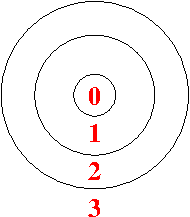
\includegraphics{cible.pdf}}
\end{minipage}
\hfill
\begin{minipage}{11.65cm}
$$\begin{tabular}{l@{ : }l@{ $\rightarrow$ }l}
0 & «~en plein dans le mille !~» & l'objectif est atteint \\
1 & «~pas mal !~» & on se rapproche de l'objectif \\
2 & «~juste au bord de la cible !~» & on est encore loin de l'objectif\\
3 & «~la cible n'est pas touchée !~» & l'objectif n'est pas atteint
\end{tabular}$$
\end{minipage}
\vspace*{2mm}

Ainsi, et pour changer de point de vue sur la notation, le contrôle 
est réussi lorsqu'on a 0 ! Il n'y a pas non plus de $1/2$ point ou de $1/4$ 
de point : le seul barême possible ne comporte que 4 niveaux : 0, 1, 2 et 3.
On ne cherche donc pas à «~grappiller~» des points : 
\begin{itemize}
\item on peut avoir 0 (objectif atteint) et avoir fait une ou deux erreurs 
	bénignes en regard de l'objectif recherché;
\item on peut avoir 3 (objectif non atteint) et avoir quelques éléments de
	réponse corrects mais sans grand rapport avec l'objectif;
\item une absence au contrôle est sanctionnée par la note 4, dite note minimale.	
\end{itemize}

Pour obtenir une note plus « classique » (ie. une note sur 20 : $n_{/20}$), il suffit
de prendre le complément à 4 de la note sur 0 ($n_{/0}$) et de le multiplier par 5 :

$$n_{/20} = (4 - n_{/0})\times 5\hfill \makebox[5.25cm]{soient les équivalences :}\hfill
\begin{array}{r|r|l}
n_{/0} & n_{/20} & \mbox{signification} \\
\hline
0 & 20 & \mbox{l'objectif est atteint}\\
1 & 15 & \mbox{on se rapproche de l'objectif}\\
2 & 10 & \mbox{on est encore loin de l'objectif}\\
3 &  5 & \mbox{l'objectif n'est pas atteint}\\
4 &  0 & \mbox{l'objectif n'a pas été visé}
\end{array}$$

Ainsi, dans ce contexte, avoir $20/20$ ne signifie pas qu'on est génial ou que c'est parfait,
cela signifie « juste » qu'on a atteint un objectif fixé, et c'est déjà beaucoup !

\subsubsection{Règles de base}
\begin{itemize}
\item Toute absence non justifiée à un contrôle (ie. justification non validée par l'administration) est sanctionnée 
par la note minimale et ne donne pas lieu à rattrapage.

\begin{quote}
Extrait du règlement des études de l'\enib : « Un étudiant absent sans justifications 
à trois évaluations en cours d'année pourra être considéré comme démissionnaire. »
\end{quote}

\item Pendant les contrôles, tous documents, téléphones, calculettes et ordinateurs personnels sont interdits. Tout manquement est sanctionnée par la note minimale et ne donne pas lieu à rattrapage.

\item Toute fraude est sanctionnée par la note minimale, ne donne pas lieu à rattrapage et
fait l'objet d'une convocation devant le conseil de discipline.
\end{itemize}

%-------------------------------------------------------------------------
\end{document}
%-------------------------------------------------------------------------
